\section{Server Architecture}
%The purpose of this section is to describe the overall architecture of the server.

% Something like:

%		Client
%		------
%Server:  IO
%       [] [] [] [] []...
%     [Game1] [Game 2] ... [Game n]   [MENU/LOGIN]
%     []  []  []  [] []...
%        [DB]

% Class diagram

% Database schema

\subsection{Database}
In this project a database was needed to keep track of all information related to users and games they are playing. The database is designed with flexibility in mind which means that the logic behind a game is responsible for interpreting the data in the database. \figref{fig:ER}\fxwarning{export new ER diagram} shows the entity relation diagram for the database without attributes. The database is structured as follows:

\begin{figure}
  \centering
  % Graphic for TeX using PGF
% \usepackage{tikz}
% The following commands are not supported in PSTricks at present
% We define them conditionally, so when they are implemented,
% this pgf file will use them.
\ifx\du\undefined
  \newlength{\du}
\fi
\setlength{\du}{15\unitlength}
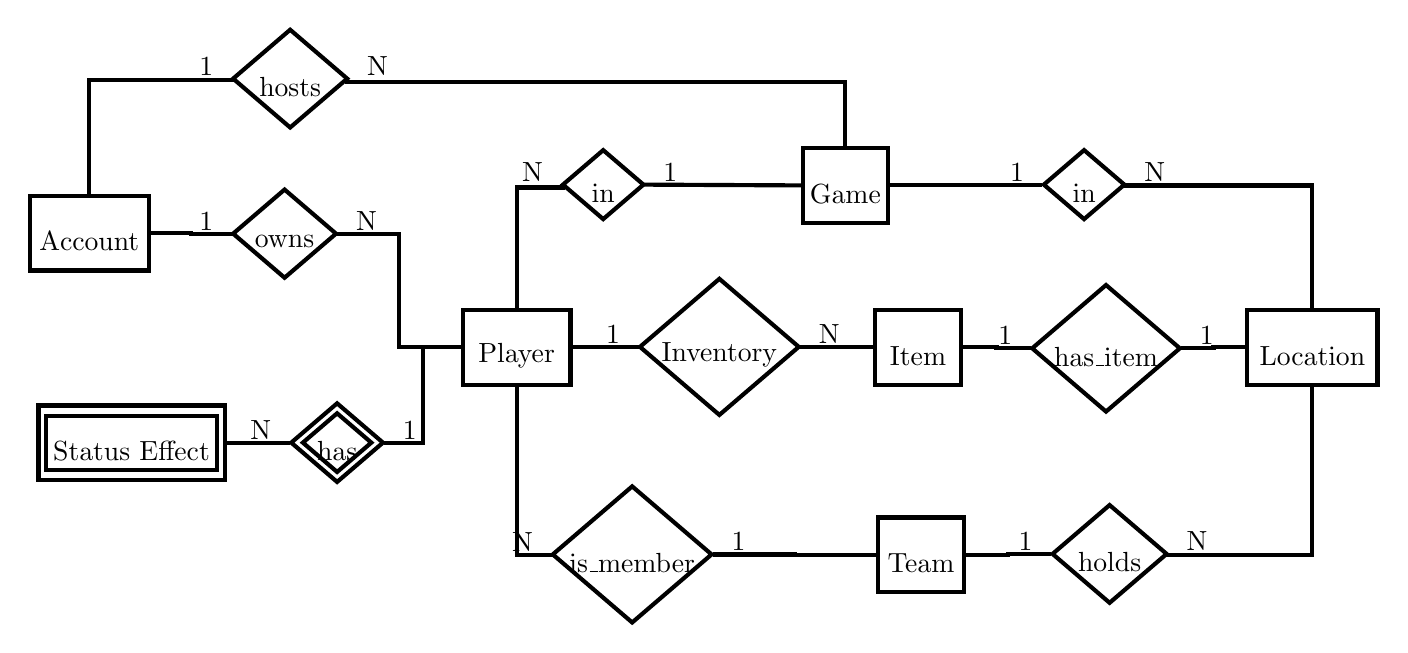
\begin{tikzpicture}
\pgftransformxscale{0.700000}
\pgftransformyscale{-1.000000}
\definecolor{dialinecolor}{rgb}{0.000000, 0.000000, 0.000000}
\pgfsetstrokecolor{dialinecolor}
\definecolor{dialinecolor}{rgb}{1.000000, 1.000000, 1.000000}
\pgfsetfillcolor{dialinecolor}
\definecolor{dialinecolor}{rgb}{1.000000, 1.000000, 1.000000}
\pgfsetfillcolor{dialinecolor}
\fill (-8.000000\du,-6.000000\du)--(-8.000000\du,-4.200000\du)--(-3.905000\du,-4.200000\du)--(-3.905000\du,-6.000000\du)--cycle;
\pgfsetlinewidth{0.100000\du}
\pgfsetdash{}{0pt}
\pgfsetmiterjoin
\definecolor{dialinecolor}{rgb}{0.000000, 0.000000, 0.000000}
\pgfsetstrokecolor{dialinecolor}
\draw (-8.000000\du,-6.000000\du)--(-8.000000\du,-4.200000\du)--(-3.905000\du,-4.200000\du)--(-3.905000\du,-6.000000\du)--cycle;
% setfont left to latex
\definecolor{dialinecolor}{rgb}{0.000000, 0.000000, 0.000000}
\pgfsetstrokecolor{dialinecolor}
\node at (-5.952500\du,-4.900000\du){Account};
\definecolor{dialinecolor}{rgb}{1.000000, 1.000000, 1.000000}
\pgfsetfillcolor{dialinecolor}
\fill (18.600000\du,-7.150000\du)--(18.600000\du,-5.350000\du)--(21.540000\du,-5.350000\du)--(21.540000\du,-7.150000\du)--cycle;
\pgfsetlinewidth{0.100000\du}
\pgfsetdash{}{0pt}
\pgfsetmiterjoin
\definecolor{dialinecolor}{rgb}{0.000000, 0.000000, 0.000000}
\pgfsetstrokecolor{dialinecolor}
\draw (18.600000\du,-7.150000\du)--(18.600000\du,-5.350000\du)--(21.540000\du,-5.350000\du)--(21.540000\du,-7.150000\du)--cycle;
% setfont left to latex
\definecolor{dialinecolor}{rgb}{0.000000, 0.000000, 0.000000}
\pgfsetstrokecolor{dialinecolor}
\node at (20.070000\du,-6.050000\du){Game};
\definecolor{dialinecolor}{rgb}{1.000000, 1.000000, 1.000000}
\pgfsetfillcolor{dialinecolor}
\fill (21.200000\du,1.750000\du)--(21.200000\du,3.550000\du)--(24.140000\du,3.550000\du)--(24.140000\du,1.750000\du)--cycle;
\pgfsetlinewidth{0.100000\du}
\pgfsetdash{}{0pt}
\pgfsetmiterjoin
\definecolor{dialinecolor}{rgb}{0.000000, 0.000000, 0.000000}
\pgfsetstrokecolor{dialinecolor}
\draw (21.200000\du,1.750000\du)--(21.200000\du,3.550000\du)--(24.140000\du,3.550000\du)--(24.140000\du,1.750000\du)--cycle;
% setfont left to latex
\definecolor{dialinecolor}{rgb}{0.000000, 0.000000, 0.000000}
\pgfsetstrokecolor{dialinecolor}
\node at (22.670000\du,2.850000\du){Team};
% setfont left to latex
\definecolor{dialinecolor}{rgb}{0.000000, 0.000000, 0.000000}
\pgfsetstrokecolor{dialinecolor}
\node[anchor=west] at (22.670000\du,2.650000\du){};
\definecolor{dialinecolor}{rgb}{1.000000, 1.000000, 1.000000}
\pgfsetfillcolor{dialinecolor}
\fill (13.000000\du,-2.360500\du)--(15.732500\du,-4.000000\du)--(18.465000\du,-2.360500\du)--(15.732500\du,-0.721000\du)--cycle;
\pgfsetlinewidth{0.100000\du}
\pgfsetdash{}{0pt}
\pgfsetmiterjoin
\definecolor{dialinecolor}{rgb}{0.000000, 0.000000, 0.000000}
\pgfsetstrokecolor{dialinecolor}
\draw (13.000000\du,-2.360500\du)--(15.732500\du,-4.000000\du)--(18.465000\du,-2.360500\du)--(15.732500\du,-0.721000\du)--cycle;
% setfont left to latex
\definecolor{dialinecolor}{rgb}{0.000000, 0.000000, 0.000000}
\pgfsetstrokecolor{dialinecolor}
\node[anchor=east] at (12.700000\du,-2.660500\du){1};
\definecolor{dialinecolor}{rgb}{0.000000, 0.000000, 0.000000}
\pgfsetstrokecolor{dialinecolor}
\node[anchor=west] at (18.765000\du,-2.660500\du){N};
\definecolor{dialinecolor}{rgb}{0.000000, 0.000000, 0.000000}
\pgfsetstrokecolor{dialinecolor}
\node at (15.732500\du,-2.160500\du){Inventory};
\definecolor{dialinecolor}{rgb}{1.000000, 1.000000, 1.000000}
\pgfsetfillcolor{dialinecolor}
\fill (21.100000\du,-3.250000\du)--(21.100000\du,-1.450000\du)--(24.040000\du,-1.450000\du)--(24.040000\du,-3.250000\du)--cycle;
\pgfsetlinewidth{0.100000\du}
\pgfsetdash{}{0pt}
\pgfsetmiterjoin
\definecolor{dialinecolor}{rgb}{0.000000, 0.000000, 0.000000}
\pgfsetstrokecolor{dialinecolor}
\draw (21.100000\du,-3.250000\du)--(21.100000\du,-1.450000\du)--(24.040000\du,-1.450000\du)--(24.040000\du,-3.250000\du)--cycle;
% setfont left to latex
\definecolor{dialinecolor}{rgb}{0.000000, 0.000000, 0.000000}
\pgfsetstrokecolor{dialinecolor}
\node at (22.570000\du,-2.150000\du){Item};
\definecolor{dialinecolor}{rgb}{1.000000, 1.000000, 1.000000}
\pgfsetfillcolor{dialinecolor}
\fill (26.500000\du,-2.325999\du)--(29.040000\du,-3.849999\du)--(31.580000\du,-2.325999\du)--(29.040000\du,-0.801999\du)--cycle;
\pgfsetlinewidth{0.100000\du}
\pgfsetdash{}{0pt}
\pgfsetmiterjoin
\definecolor{dialinecolor}{rgb}{0.000000, 0.000000, 0.000000}
\pgfsetstrokecolor{dialinecolor}
\draw (26.500000\du,-2.325999\du)--(29.040000\du,-3.849999\du)--(31.580000\du,-2.325999\du)--(29.040000\du,-0.801999\du)--cycle;
% setfont left to latex
\definecolor{dialinecolor}{rgb}{0.000000, 0.000000, 0.000000}
\pgfsetstrokecolor{dialinecolor}
\node[anchor=east] at (26.200000\du,-2.625999\du){1};
\definecolor{dialinecolor}{rgb}{0.000000, 0.000000, 0.000000}
\pgfsetstrokecolor{dialinecolor}
\node[anchor=west] at (31.880000\du,-2.625999\du){1};
\definecolor{dialinecolor}{rgb}{0.000000, 0.000000, 0.000000}
\pgfsetstrokecolor{dialinecolor}
\node at (29.040000\du,-2.125999\du){has\_item};
\definecolor{dialinecolor}{rgb}{1.000000, 1.000000, 1.000000}
\pgfsetfillcolor{dialinecolor}
\fill (33.900000\du,-3.250000\du)--(33.900000\du,-1.450000\du)--(38.380000\du,-1.450000\du)--(38.380000\du,-3.250000\du)--cycle;
\pgfsetlinewidth{0.100000\du}
\pgfsetdash{}{0pt}
\pgfsetmiterjoin
\definecolor{dialinecolor}{rgb}{0.000000, 0.000000, 0.000000}
\pgfsetstrokecolor{dialinecolor}
\draw (33.900000\du,-3.250000\du)--(33.900000\du,-1.450000\du)--(38.380000\du,-1.450000\du)--(38.380000\du,-3.250000\du)--cycle;
% setfont left to latex
\definecolor{dialinecolor}{rgb}{0.000000, 0.000000, 0.000000}
\pgfsetstrokecolor{dialinecolor}
\node at (36.140000\du,-2.150000\du){Location};
\definecolor{dialinecolor}{rgb}{1.000000, 1.000000, 1.000000}
\pgfsetfillcolor{dialinecolor}
\fill (27.200004\du,2.627500\du)--(29.162504\du,1.450000\du)--(31.125004\du,2.627500\du)--(29.162504\du,3.805000\du)--cycle;
\pgfsetlinewidth{0.100000\du}
\pgfsetdash{}{0pt}
\pgfsetmiterjoin
\definecolor{dialinecolor}{rgb}{0.000000, 0.000000, 0.000000}
\pgfsetstrokecolor{dialinecolor}
\draw (27.200004\du,2.627500\du)--(29.162504\du,1.450000\du)--(31.125004\du,2.627500\du)--(29.162504\du,3.805000\du)--cycle;
% setfont left to latex
\definecolor{dialinecolor}{rgb}{0.000000, 0.000000, 0.000000}
\pgfsetstrokecolor{dialinecolor}
\node[anchor=east] at (26.900004\du,2.327500\du){1};
\definecolor{dialinecolor}{rgb}{0.000000, 0.000000, 0.000000}
\pgfsetstrokecolor{dialinecolor}
\node[anchor=west] at (31.425004\du,2.327500\du){N};
\definecolor{dialinecolor}{rgb}{0.000000, 0.000000, 0.000000}
\pgfsetstrokecolor{dialinecolor}
\node at (29.162504\du,2.827500\du){holds};
\definecolor{dialinecolor}{rgb}{1.000000, 1.000000, 1.000000}
\pgfsetfillcolor{dialinecolor}
\fill (26.900004\du,-6.268999\du)--(28.285004\du,-7.099999\du)--(29.670004\du,-6.268999\du)--(28.285004\du,-5.437999\du)--cycle;
\pgfsetlinewidth{0.100000\du}
\pgfsetdash{}{0pt}
\pgfsetmiterjoin
\definecolor{dialinecolor}{rgb}{0.000000, 0.000000, 0.000000}
\pgfsetstrokecolor{dialinecolor}
\draw (26.900004\du,-6.268999\du)--(28.285004\du,-7.099999\du)--(29.670004\du,-6.268999\du)--(28.285004\du,-5.437999\du)--cycle;
% setfont left to latex
\definecolor{dialinecolor}{rgb}{0.000000, 0.000000, 0.000000}
\pgfsetstrokecolor{dialinecolor}
\node[anchor=east] at (26.600004\du,-6.568999\du){1};
\definecolor{dialinecolor}{rgb}{0.000000, 0.000000, 0.000000}
\pgfsetstrokecolor{dialinecolor}
\node[anchor=west] at (29.970004\du,-6.568999\du){N};
\definecolor{dialinecolor}{rgb}{0.000000, 0.000000, 0.000000}
\pgfsetstrokecolor{dialinecolor}
\node at (28.285004\du,-6.068999\du){in};
\definecolor{dialinecolor}{rgb}{1.000000, 1.000000, 1.000000}
\pgfsetfillcolor{dialinecolor}
\fill (-1.000000\du,-8.822500\du)--(0.962500\du,-10.000000\du)--(2.925000\du,-8.822500\du)--(0.962500\du,-7.645000\du)--cycle;
\pgfsetlinewidth{0.100000\du}
\pgfsetdash{}{0pt}
\pgfsetmiterjoin
\definecolor{dialinecolor}{rgb}{0.000000, 0.000000, 0.000000}
\pgfsetstrokecolor{dialinecolor}
\draw (-1.000000\du,-8.822500\du)--(0.962500\du,-10.000000\du)--(2.925000\du,-8.822500\du)--(0.962500\du,-7.645000\du)--cycle;
% setfont left to latex
\definecolor{dialinecolor}{rgb}{0.000000, 0.000000, 0.000000}
\pgfsetstrokecolor{dialinecolor}
\node[anchor=east] at (-1.300000\du,-9.122500\du){1};
\definecolor{dialinecolor}{rgb}{0.000000, 0.000000, 0.000000}
\pgfsetstrokecolor{dialinecolor}
\node[anchor=west] at (3.225000\du,-9.122500\du){N};
\definecolor{dialinecolor}{rgb}{0.000000, 0.000000, 0.000000}
\pgfsetstrokecolor{dialinecolor}
\node at (0.962500\du,-8.622500\du){hosts};
\definecolor{dialinecolor}{rgb}{1.000000, 1.000000, 1.000000}
\pgfsetfillcolor{dialinecolor}
\fill (6.900000\du,-3.250001\du)--(6.900000\du,-1.450001\du)--(10.610000\du,-1.450001\du)--(10.610000\du,-3.250001\du)--cycle;
\pgfsetlinewidth{0.100000\du}
\pgfsetdash{}{0pt}
\pgfsetmiterjoin
\definecolor{dialinecolor}{rgb}{0.000000, 0.000000, 0.000000}
\pgfsetstrokecolor{dialinecolor}
\draw (6.900000\du,-3.250001\du)--(6.900000\du,-1.450001\du)--(10.610000\du,-1.450001\du)--(10.610000\du,-3.250001\du)--cycle;
% setfont left to latex
\definecolor{dialinecolor}{rgb}{0.000000, 0.000000, 0.000000}
\pgfsetstrokecolor{dialinecolor}
\node at (8.755000\du,-2.150001\du){Player};
\definecolor{dialinecolor}{rgb}{1.000000, 1.000000, 1.000000}
\pgfsetfillcolor{dialinecolor}
\fill (-1.000000\du,-5.088000\du)--(0.770000\du,-6.150000\du)--(2.540000\du,-5.088000\du)--(0.770000\du,-4.026000\du)--cycle;
\pgfsetlinewidth{0.100000\du}
\pgfsetdash{}{0pt}
\pgfsetmiterjoin
\definecolor{dialinecolor}{rgb}{0.000000, 0.000000, 0.000000}
\pgfsetstrokecolor{dialinecolor}
\draw (-1.000000\du,-5.088000\du)--(0.770000\du,-6.150000\du)--(2.540000\du,-5.088000\du)--(0.770000\du,-4.026000\du)--cycle;
% setfont left to latex
\definecolor{dialinecolor}{rgb}{0.000000, 0.000000, 0.000000}
\pgfsetstrokecolor{dialinecolor}
\node[anchor=east] at (-1.300000\du,-5.388000\du){1};
\definecolor{dialinecolor}{rgb}{0.000000, 0.000000, 0.000000}
\pgfsetstrokecolor{dialinecolor}
\node[anchor=west] at (2.840000\du,-5.388000\du){N};
\definecolor{dialinecolor}{rgb}{0.000000, 0.000000, 0.000000}
\pgfsetstrokecolor{dialinecolor}
\node at (0.770000\du,-4.888000\du){owns};
\definecolor{dialinecolor}{rgb}{1.000000, 1.000000, 1.000000}
\pgfsetfillcolor{dialinecolor}
\fill (10.350000\du,-6.269000\du)--(11.735000\du,-7.100000\du)--(13.120000\du,-6.269000\du)--(11.735000\du,-5.438000\du)--cycle;
\pgfsetlinewidth{0.100000\du}
\pgfsetdash{}{0pt}
\pgfsetmiterjoin
\definecolor{dialinecolor}{rgb}{0.000000, 0.000000, 0.000000}
\pgfsetstrokecolor{dialinecolor}
\draw (10.350000\du,-6.269000\du)--(11.735000\du,-7.100000\du)--(13.120000\du,-6.269000\du)--(11.735000\du,-5.438000\du)--cycle;
% setfont left to latex
\definecolor{dialinecolor}{rgb}{0.000000, 0.000000, 0.000000}
\pgfsetstrokecolor{dialinecolor}
\node[anchor=east] at (10.050000\du,-6.569000\du){N};
\definecolor{dialinecolor}{rgb}{0.000000, 0.000000, 0.000000}
\pgfsetstrokecolor{dialinecolor}
\node[anchor=west] at (13.420000\du,-6.569000\du){1};
\definecolor{dialinecolor}{rgb}{0.000000, 0.000000, 0.000000}
\pgfsetstrokecolor{dialinecolor}
\node at (11.735000\du,-6.069000\du){in};
\pgfsetlinewidth{0.100000\du}
\pgfsetdash{}{0pt}
\pgfsetdash{}{0pt}
\pgfsetbuttcap
{
\definecolor{dialinecolor}{rgb}{0.000000, 0.000000, 0.000000}
\pgfsetfillcolor{dialinecolor}
% was here!!!
\definecolor{dialinecolor}{rgb}{0.000000, 0.000000, 0.000000}
\pgfsetstrokecolor{dialinecolor}
\draw (13.120000\du,-6.269000\du)--(18.600000\du,-6.250000\du);
}
\definecolor{dialinecolor}{rgb}{1.000000, 1.000000, 1.000000}
\pgfsetfillcolor{dialinecolor}
\fill (10.000000\du,2.639500\du)--(12.732500\du,1.000000\du)--(15.465000\du,2.639500\du)--(12.732500\du,4.279000\du)--cycle;
\pgfsetlinewidth{0.100000\du}
\pgfsetdash{}{0pt}
\pgfsetmiterjoin
\definecolor{dialinecolor}{rgb}{0.000000, 0.000000, 0.000000}
\pgfsetstrokecolor{dialinecolor}
\draw (10.000000\du,2.639500\du)--(12.732500\du,1.000000\du)--(15.465000\du,2.639500\du)--(12.732500\du,4.279000\du)--cycle;
% setfont left to latex
\definecolor{dialinecolor}{rgb}{0.000000, 0.000000, 0.000000}
\pgfsetstrokecolor{dialinecolor}
\node[anchor=east] at (9.700000\du,2.339500\du){N};
\definecolor{dialinecolor}{rgb}{0.000000, 0.000000, 0.000000}
\pgfsetstrokecolor{dialinecolor}
\node[anchor=west] at (15.765000\du,2.339500\du){1};
\definecolor{dialinecolor}{rgb}{0.000000, 0.000000, 0.000000}
\pgfsetstrokecolor{dialinecolor}
\node at (12.732500\du,2.839500\du){is\_member};
\definecolor{dialinecolor}{rgb}{1.000000, 1.000000, 1.000000}
\pgfsetfillcolor{dialinecolor}
\fill (-7.700000\du,-0.949999\du)--(-7.700000\du,0.850001\du)--(-1.295000\du,0.850001\du)--(-1.295000\du,-0.949999\du)--cycle;
\pgfsetlinewidth{0.100000\du}
\pgfsetdash{}{0pt}
\pgfsetmiterjoin
\definecolor{dialinecolor}{rgb}{0.000000, 0.000000, 0.000000}
\pgfsetstrokecolor{dialinecolor}
\draw (-7.700000\du,-0.949999\du)--(-7.700000\du,0.850001\du)--(-1.295000\du,0.850001\du)--(-1.295000\du,-0.949999\du)--cycle;
\definecolor{dialinecolor}{rgb}{0.000000, 0.000000, 0.000000}
\pgfsetstrokecolor{dialinecolor}
\draw (-7.450000\du,-0.699999\du)--(-7.450000\du,0.600001\du)--(-1.545000\du,0.600001\du)--(-1.545000\du,-0.699999\du)--cycle;
% setfont left to latex
\definecolor{dialinecolor}{rgb}{0.000000, 0.000000, 0.000000}
\pgfsetstrokecolor{dialinecolor}
\node at (-4.497500\du,0.150001\du){Status Effect};
\definecolor{dialinecolor}{rgb}{1.000000, 1.000000, 1.000000}
\pgfsetfillcolor{dialinecolor}
\fill (1.000000\du,-0.053500\du)--(2.577500\du,-1.000000\du)--(4.155000\du,-0.053500\du)--(2.577500\du,0.893000\du)--cycle;
\pgfsetlinewidth{0.100000\du}
\pgfsetdash{}{0pt}
\pgfsetmiterjoin
\definecolor{dialinecolor}{rgb}{0.000000, 0.000000, 0.000000}
\pgfsetstrokecolor{dialinecolor}
\draw (1.000000\du,-0.053500\du)--(2.577500\du,-1.000000\du)--(4.155000\du,-0.053500\du)--(2.577500\du,0.893000\du)--cycle;
\definecolor{dialinecolor}{rgb}{0.000000, 0.000000, 0.000000}
\pgfsetstrokecolor{dialinecolor}
\draw (1.400000\du,-0.053500\du)--(2.577500\du,-0.760000\du)--(3.755000\du,-0.053500\du)--(2.577500\du,0.653000\du)--cycle;
% setfont left to latex
\definecolor{dialinecolor}{rgb}{0.000000, 0.000000, 0.000000}
\pgfsetstrokecolor{dialinecolor}
\node[anchor=east] at (0.700000\du,-0.353500\du){N};
\definecolor{dialinecolor}{rgb}{0.000000, 0.000000, 0.000000}
\pgfsetstrokecolor{dialinecolor}
\node[anchor=west] at (4.455000\du,-0.353500\du){1};
\definecolor{dialinecolor}{rgb}{0.000000, 0.000000, 0.000000}
\pgfsetstrokecolor{dialinecolor}
\node at (2.577500\du,0.146500\du){has};
\pgfsetlinewidth{0.100000\du}
\pgfsetdash{}{0pt}
\pgfsetdash{}{0pt}
\pgfsetmiterjoin
\pgfsetbuttcap
{
\definecolor{dialinecolor}{rgb}{0.000000, 0.000000, 0.000000}
\pgfsetfillcolor{dialinecolor}
% was here!!!
{\pgfsetcornersarced{\pgfpoint{0.000000\du}{0.000000\du}}\definecolor{dialinecolor}{rgb}{0.000000, 0.000000, 0.000000}
\pgfsetstrokecolor{dialinecolor}
\draw (20.070000\du,-7.150000\du)--(20.070000\du,-8.749106\du)--(2.925000\du,-8.749106\du)--(2.925000\du,-8.822500\du);
}}
\pgfsetlinewidth{0.100000\du}
\pgfsetdash{}{0pt}
\pgfsetdash{}{0pt}
\pgfsetmiterjoin
\pgfsetbuttcap
{
\definecolor{dialinecolor}{rgb}{0.000000, 0.000000, 0.000000}
\pgfsetfillcolor{dialinecolor}
% was here!!!
{\pgfsetcornersarced{\pgfpoint{0.000000\du}{0.000000\du}}\definecolor{dialinecolor}{rgb}{0.000000, 0.000000, 0.000000}
\pgfsetstrokecolor{dialinecolor}
\draw (-1.000000\du,-8.822500\du)--(-1.000000\du,-8.799106\du)--(-5.952500\du,-8.799106\du)--(-5.952500\du,-6.000000\du);
}}
\pgfsetlinewidth{0.100000\du}
\pgfsetdash{}{0pt}
\pgfsetdash{}{0pt}
\pgfsetmiterjoin
\pgfsetbuttcap
{
\definecolor{dialinecolor}{rgb}{0.000000, 0.000000, 0.000000}
\pgfsetfillcolor{dialinecolor}
% was here!!!
{\pgfsetcornersarced{\pgfpoint{0.000000\du}{0.000000\du}}\definecolor{dialinecolor}{rgb}{0.000000, 0.000000, 0.000000}
\pgfsetstrokecolor{dialinecolor}
\draw (-1.000000\du,-5.088000\du)--(-2.452500\du,-5.088000\du)--(-2.452500\du,-5.100000\du)--(-3.905000\du,-5.100000\du);
}}
\pgfsetlinewidth{0.100000\du}
\pgfsetdash{}{0pt}
\pgfsetdash{}{0pt}
\pgfsetmiterjoin
\pgfsetbuttcap
{
\definecolor{dialinecolor}{rgb}{0.000000, 0.000000, 0.000000}
\pgfsetfillcolor{dialinecolor}
% was here!!!
{\pgfsetcornersarced{\pgfpoint{0.000000\du}{0.000000\du}}\definecolor{dialinecolor}{rgb}{0.000000, 0.000000, 0.000000}
\pgfsetstrokecolor{dialinecolor}
\draw (2.540000\du,-5.088000\du)--(4.720000\du,-5.088000\du)--(4.720000\du,-2.350001\du)--(6.900000\du,-2.350001\du);
}}
\pgfsetlinewidth{0.100000\du}
\pgfsetdash{}{0pt}
\pgfsetdash{}{0pt}
\pgfsetmiterjoin
\pgfsetbuttcap
{
\definecolor{dialinecolor}{rgb}{0.000000, 0.000000, 0.000000}
\pgfsetfillcolor{dialinecolor}
% was here!!!
{\pgfsetcornersarced{\pgfpoint{0.000000\du}{0.000000\du}}\definecolor{dialinecolor}{rgb}{0.000000, 0.000000, 0.000000}
\pgfsetstrokecolor{dialinecolor}
\draw (10.350000\du,-6.269000\du)--(10.350000\du,-6.199108\du)--(8.755000\du,-6.199108\du)--(8.755000\du,-3.299591\du);
}}
\pgfsetlinewidth{0.100000\du}
\pgfsetdash{}{0pt}
\pgfsetdash{}{0pt}
\pgfsetmiterjoin
\pgfsetbuttcap
{
\definecolor{dialinecolor}{rgb}{0.000000, 0.000000, 0.000000}
\pgfsetfillcolor{dialinecolor}
% was here!!!
{\pgfsetcornersarced{\pgfpoint{0.000000\du}{0.000000\du}}\definecolor{dialinecolor}{rgb}{0.000000, 0.000000, 0.000000}
\pgfsetstrokecolor{dialinecolor}
\draw (6.849535\du,-2.350001\du)--(5.527070\du,-2.350001\du)--(5.527070\du,-0.053500\du)--(4.204606\du,-0.053500\du);
}}
\pgfsetlinewidth{0.100000\du}
\pgfsetdash{}{0pt}
\pgfsetdash{}{0pt}
\pgfsetmiterjoin
\pgfsetbuttcap
{
\definecolor{dialinecolor}{rgb}{0.000000, 0.000000, 0.000000}
\pgfsetfillcolor{dialinecolor}
% was here!!!
{\pgfsetcornersarced{\pgfpoint{0.000000\du}{0.000000\du}}\definecolor{dialinecolor}{rgb}{0.000000, 0.000000, 0.000000}
\pgfsetstrokecolor{dialinecolor}
\draw (12.952405\du,-2.360500\du)--(11.806435\du,-2.360500\du)--(11.806435\du,-2.350001\du)--(10.660465\du,-2.350001\du);
}}
\pgfsetlinewidth{0.100000\du}
\pgfsetdash{}{0pt}
\pgfsetdash{}{0pt}
\pgfsetmiterjoin
\pgfsetbuttcap
{
\definecolor{dialinecolor}{rgb}{0.000000, 0.000000, 0.000000}
\pgfsetfillcolor{dialinecolor}
% was here!!!
{\pgfsetcornersarced{\pgfpoint{0.000000\du}{0.000000\du}}\definecolor{dialinecolor}{rgb}{0.000000, 0.000000, 0.000000}
\pgfsetstrokecolor{dialinecolor}
\draw (21.049629\du,-2.350000\du)--(19.781112\du,-2.350000\du)--(19.781112\du,-2.360500\du)--(18.512595\du,-2.360500\du);
}}
\pgfsetlinewidth{0.100000\du}
\pgfsetdash{}{0pt}
\pgfsetdash{}{0pt}
\pgfsetmiterjoin
\pgfsetbuttcap
{
\definecolor{dialinecolor}{rgb}{0.000000, 0.000000, 0.000000}
\pgfsetfillcolor{dialinecolor}
% was here!!!
{\pgfsetcornersarced{\pgfpoint{0.000000\du}{0.000000\du}}\definecolor{dialinecolor}{rgb}{0.000000, 0.000000, 0.000000}
\pgfsetstrokecolor{dialinecolor}
\draw (24.090371\du,-2.350000\du)--(25.271496\du,-2.350000\du)--(25.271496\du,-2.325999\du)--(26.452622\du,-2.325999\du);
}}
\pgfsetlinewidth{0.100000\du}
\pgfsetdash{}{0pt}
\pgfsetdash{}{0pt}
\pgfsetmiterjoin
\pgfsetbuttcap
{
\definecolor{dialinecolor}{rgb}{0.000000, 0.000000, 0.000000}
\pgfsetfillcolor{dialinecolor}
% was here!!!
{\pgfsetcornersarced{\pgfpoint{0.000000\du}{0.000000\du}}\definecolor{dialinecolor}{rgb}{0.000000, 0.000000, 0.000000}
\pgfsetstrokecolor{dialinecolor}
\draw (21.590371\du,-6.250000\du)--(24.220066\du,-6.250000\du)--(24.220066\du,-6.268999\du)--(26.849760\du,-6.268999\du);
}}
\pgfsetlinewidth{0.100000\du}
\pgfsetdash{}{0pt}
\pgfsetdash{}{0pt}
\pgfsetmiterjoin
\pgfsetbuttcap
{
\definecolor{dialinecolor}{rgb}{0.000000, 0.000000, 0.000000}
\pgfsetfillcolor{dialinecolor}
% was here!!!
{\pgfsetcornersarced{\pgfpoint{0.000000\du}{0.000000\du}}\definecolor{dialinecolor}{rgb}{0.000000, 0.000000, 0.000000}
\pgfsetstrokecolor{dialinecolor}
\draw (36.140000\du,-3.250000\du)--(36.140000\du,-6.249108\du)--(29.670004\du,-6.249108\du)--(29.670004\du,-6.268999\du);
}}
\pgfsetlinewidth{0.100000\du}
\pgfsetdash{}{0pt}
\pgfsetdash{}{0pt}
\pgfsetmiterjoin
\pgfsetbuttcap
{
\definecolor{dialinecolor}{rgb}{0.000000, 0.000000, 0.000000}
\pgfsetfillcolor{dialinecolor}
% was here!!!
{\pgfsetcornersarced{\pgfpoint{0.000000\du}{0.000000\du}}\definecolor{dialinecolor}{rgb}{0.000000, 0.000000, 0.000000}
\pgfsetstrokecolor{dialinecolor}
\draw (31.627378\du,-2.325999\du)--(32.738549\du,-2.325999\du)--(32.738549\du,-2.350000\du)--(33.849721\du,-2.350000\du);
}}
\pgfsetlinewidth{0.100000\du}
\pgfsetdash{}{0pt}
\pgfsetdash{}{0pt}
\pgfsetmiterjoin
\pgfsetbuttcap
{
\definecolor{dialinecolor}{rgb}{0.000000, 0.000000, 0.000000}
\pgfsetfillcolor{dialinecolor}
% was here!!!
{\pgfsetcornersarced{\pgfpoint{0.000000\du}{0.000000\du}}\definecolor{dialinecolor}{rgb}{0.000000, 0.000000, 0.000000}
\pgfsetstrokecolor{dialinecolor}
\draw (21.149629\du,2.650000\du)--(18.331112\du,2.650000\du)--(18.331112\du,2.639500\du)--(15.512595\du,2.639500\du);
}}
\pgfsetlinewidth{0.100000\du}
\pgfsetdash{}{0pt}
\pgfsetdash{}{0pt}
\pgfsetmiterjoin
\pgfsetbuttcap
{
\definecolor{dialinecolor}{rgb}{0.000000, 0.000000, 0.000000}
\pgfsetfillcolor{dialinecolor}
% was here!!!
{\pgfsetcornersarced{\pgfpoint{0.000000\du}{0.000000\du}}\definecolor{dialinecolor}{rgb}{0.000000, 0.000000, 0.000000}
\pgfsetstrokecolor{dialinecolor}
\draw (24.190371\du,2.650000\du)--(25.672778\du,2.650000\du)--(25.672778\du,2.627500\du)--(27.155184\du,2.627500\du);
}}
\pgfsetlinewidth{0.100000\du}
\pgfsetdash{}{0pt}
\pgfsetdash{}{0pt}
\pgfsetmiterjoin
\pgfsetbuttcap
{
\definecolor{dialinecolor}{rgb}{0.000000, 0.000000, 0.000000}
\pgfsetfillcolor{dialinecolor}
% was here!!!
{\pgfsetcornersarced{\pgfpoint{0.000000\du}{0.000000\du}}\definecolor{dialinecolor}{rgb}{0.000000, 0.000000, 0.000000}
\pgfsetstrokecolor{dialinecolor}
\draw (-1.244603\du,-0.049999\du)--(-0.147104\du,-0.049999\du)--(-0.147104\du,-0.053500\du)--(0.950394\du,-0.053500\du);
}}
\pgfsetlinewidth{0.100000\du}
\pgfsetdash{}{0pt}
\pgfsetdash{}{0pt}
\pgfsetmiterjoin
\pgfsetbuttcap
{
\definecolor{dialinecolor}{rgb}{0.000000, 0.000000, 0.000000}
\pgfsetfillcolor{dialinecolor}
% was here!!!
{\pgfsetcornersarced{\pgfpoint{0.000000\du}{0.000000\du}}\definecolor{dialinecolor}{rgb}{0.000000, 0.000000, 0.000000}
\pgfsetstrokecolor{dialinecolor}
\draw (8.755000\du,-1.399820\du)--(8.755000\du,2.650885\du)--(10.000000\du,2.650885\du)--(10.000000\du,2.639500\du);
}}
\pgfsetlinewidth{0.100000\du}
\pgfsetdash{}{0pt}
\pgfsetdash{}{0pt}
\pgfsetmiterjoin
\pgfsetbuttcap
{
\definecolor{dialinecolor}{rgb}{0.000000, 0.000000, 0.000000}
\pgfsetfillcolor{dialinecolor}
% was here!!!
{\pgfsetcornersarced{\pgfpoint{0.000000\du}{0.000000\du}}\definecolor{dialinecolor}{rgb}{0.000000, 0.000000, 0.000000}
\pgfsetstrokecolor{dialinecolor}
\draw (36.140000\du,-1.399820\du)--(36.140000\du,2.650885\du)--(31.125004\du,2.650885\du)--(31.125004\du,2.627500\du);
}}
\end{tikzpicture}
  
  \caption{ER Diagram.}
  \label{fig:ER}
\end{figure}




\paragraph{Account}
The Account entity represent the users in the system. An account can host games represented by the host relation and take part in games represented as owning a player in a particular game.

\paragraph{Player}
This entity represents a user playing in a game. A player can hold items, have status effects and be a member of a team represented by Inventory, has(Status Effect) and Team(is\_member) respectively. The player entity also contains score and location etc. for a particular player in a game.

\paragraph{Game}
This entity represent games either \textit{starting up}, \textit{in progress} or \textit{ended}.

\paragraph{Status Effect}
Effects on a player is represented by this entity. An effect could be \textit{disabled until time} on a particular player. Status Effects have an effect type which the game logic is responsible for defining.

\paragraph{Team}
Players can be members of teams in a game, though a player is not required to be on a team to allow free for all game modes.

\paragraph{Item}
Items represent any object in the inventory of players or on a location in the game world. Items can be anything from objects players can "pick up" to a capture-able area in the game world. The attributes and behavior of items are defined by game logic.

\paragraph{Location}
A location is an item in the game world that can belong to a team. To own a location, a team must take it first.

\subsection{Game thread-pool}
The game thread-pool is a collection of active game thread-instances, uniquely identified by a game-Id.

The game thread-pool is used as a handle to the game threads, and allows dynamic call to the desired game through method-parametrization. 

\subsection{Game thread}
\paragraph{Starting a game}
A game thread will be initialised and started when a user requests to host a game. A game will be assigned a game-id by the server, user-specified settings for hosting the game will be initialised and the game will be created in the database. 

When the server initialises each setting, it calls a method within the game thread-class. These methods calls the database-controller to change the state of the game in the database. These settings are:
\begin{itemize}
\item Game-privacy (Public or private game)
\item Number of teams
\item Game start-time
\item Game end-time
\item Game-boundary NorthWest GPS-coordinate
\item Game-boundary SouthEast GPS-coordinate
\end{itemize}

\paragraph{Updating a game}
Updates to a game can be split into two groups. One group is specific changes to a game, like inviting a new player or firing a gun. Another group is updating a players position when moving around in the game.

Updating a players position is trivial. The game thread receives a game-id, player-id and a new position. It calls the database-controller to store the new position in the database.

When performing an action like firing a gun, the server will have to fetch the gunman's position and the victim's position. It will then calculate if the range of the fired weapon allows the victim to be hit. If the shot is successful it will return that to the player, if the shot is unsuccessful it will return that the victim is out of range. 

All updates to change the state of a game will be in the game thread-class. This class will need to contain methods for all the in-game functionality. 

\paragraph{Closing a game}
When a game ends, the call will come from the timer thread. This will ask the game thread to clean up what is has stored in the database, and return a status message. The timer thread will then continue to close the game thread. 



